\documentclass[aspectratio=169]{beamer}

\usetheme{Boadilla}
\usefonttheme{professionalfonts}
\setbeamertemplate{navigation symbols}{}
\setbeamertemplate{itemize items}[circle]
\setbeamertemplate{enumerate items}[default]
\setbeamertemplate{headline}{}

\usepackage[utf8]{inputenc}
\usepackage[T1]{fontenc}
\usepackage{lmodern}
\usepackage{amsmath}
\usepackage{booktabs}
\usepackage{tabularx}
\usepackage{array}
\usepackage{hyperref}
\usepackage[strings]{underscore}
\usepackage{listings}
\usepackage{tikz}
\usetikzlibrary{arrows.meta,positioning,fit,calc,shapes.geometric}
\usepackage{xcolor}

\definecolor{courseblue}{HTML}{12355B}
\definecolor{coursegold}{HTML}{C98A2E}
\definecolor{courseice}{HTML}{EEF3F8}
\definecolor{coursegreen}{HTML}{2F6B4F}
\definecolor{coursegray}{HTML}{4B5563}
\definecolor{codebg}{HTML}{F7F9FC}
\definecolor{codecomment}{HTML}{5E6C84}
\definecolor{codestring}{HTML}{0B6E4F}

\setbeamercolor{palette primary}{bg=courseblue,fg=white}
\setbeamercolor{palette secondary}{bg=coursegold,fg=white}
\setbeamercolor{palette tertiary}{bg=courseblue,fg=white}
\setbeamercolor{palette quaternary}{bg=coursegold,fg=white}
\setbeamercolor{structure}{fg=courseblue}
\setbeamercolor{frametitle}{bg=courseice,fg=courseblue}
\setbeamercolor{title}{fg=courseblue}
\setbeamercolor{block title}{bg=courseblue,fg=white}
\setbeamercolor{block body}{bg=courseice,fg=black}
\setbeamercolor{normal text}{fg=black,bg=white}
\setbeamercolor{alerted text}{fg=coursegold}

\setbeamerfont{footline}{size=\scriptsize}

\setbeamertemplate{footline}{
  \leavevmode
  \hbox{
    \begin{beamercolorbox}[wd=.33\paperwidth,ht=2.8ex,dp=1.2ex,leftskip=0.8em]{palette primary}%
      University of Trieste
    \end{beamercolorbox}%
    \begin{beamercolorbox}[wd=.49\paperwidth,ht=2.8ex,dp=1.2ex,center]{palette tertiary}%
      \coursename{} \textbar{} \coursecode
    \end{beamercolorbox}%
    \begin{beamercolorbox}[wd=.18\paperwidth,ht=2.8ex,dp=1.2ex,right,rightskip=0.8em]{palette secondary}%
      \insertframenumber{} / \inserttotalframenumber
    \end{beamercolorbox}%
  }
}

\hypersetup{
  colorlinks=true,
  linkcolor=courseblue,
  urlcolor=coursegreen
}

\lstdefinestyle{coursepython}{
  language=Python,
  basicstyle=\ttfamily\footnotesize,
  keywordstyle=\color{courseblue}\bfseries,
  commentstyle=\color{codecomment}\itshape,
  stringstyle=\color{codestring},
  showstringspaces=false,
  columns=fullflexible,
  keepspaces=true,
  frame=single,
  framerule=0.6pt,
  rulecolor=\color{courseblue},
  backgroundcolor=\color{codebg},
  xleftmargin=0.4em,
  xrightmargin=0.4em,
  aboveskip=0.4em,
  belowskip=0.2em
}

\newcommand{\coursename}{Data-driven Systems Engineering}
\newcommand{\coursecode}{440MI / 305SM}
\newcommand{\coursefooter}{}

\newcommand{\learninggoals}[1]{
  \begin{block}{Learning goals}
  #1
  \end{block}
}

\newcommand{\repoactivity}[1]{
  \begin{block}{Repo activity}
  #1
  \end{block}
}

\newcommand{\readinglist}[1]{
  \begin{block}{Papers and materials}
  {\footnotesize #1}
  \end{block}
}

\newcommand{\coursecontextframe}[5]{
  \begin{frame}{Course Map and Running Cases}
  \centering
  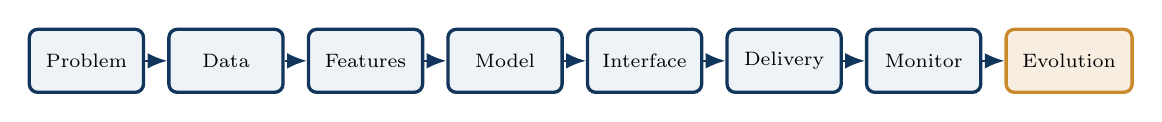
\begin{tikzpicture}[node distance=0.28cm]
  \node[flowbox, minimum width=1.45cm, minimum height=0.8cm] (problem) {\scriptsize Problem};
  \node[flowbox, minimum width=1.45cm, minimum height=0.8cm, right=of problem] (data) {\scriptsize Data};
  \node[flowbox, minimum width=1.45cm, minimum height=0.8cm, right=of data] (features) {\scriptsize Features};
  \node[flowbox, minimum width=1.45cm, minimum height=0.8cm, right=of features] (model) {\scriptsize Model};
  \node[flowbox, minimum width=1.45cm, minimum height=0.8cm, right=of model] (interface) {\scriptsize Interface};
  \node[flowbox, minimum width=1.45cm, minimum height=0.8cm, right=of interface] (delivery) {\scriptsize Delivery};
  \node[flowbox, minimum width=1.45cm, minimum height=0.8cm, right=of delivery] (monitor) {\scriptsize Monitor};
  \node[accentbox, minimum width=1.6cm, minimum height=0.8cm, right=of monitor] (evolution) {\scriptsize Evolution};
  \foreach \a/\b in {problem/data,data/features,features/model,model/interface,interface/delivery,delivery/monitor,monitor/evolution} {
    \draw[arrow] (\a) -- (\b);
  }
  \end{tikzpicture}

  \vspace{0.5em}
  \begin{block}{Today in the course}
  \textbf{Focus:} #1

  \textbf{Bridge:} #2
  \end{block}

  \begin{columns}[T]
  \column{0.48\textwidth}
  \begin{block}{Fraud case}
  {\footnotesize #3}
  \end{block}
  \column{0.48\textwidth}
  \begin{block}{Pasteurization case}
  {\footnotesize #4}
  \end{block}
  \end{columns}

  \vspace{0.3em}
  {\footnotesize \textbf{Course thread:} #5}
  \coursefooter
  \end{frame}
}

\newcommand{\classclosingframe}[4]{
  \begin{frame}{From This Class to the Next}
  \begin{block}{What stays with us}
  #1
  \end{block}

  \begin{columns}[T]
  \column{0.48\textwidth}
  \begin{block}{Project use}
  {\footnotesize #2}
  \end{block}
  \column{0.48\textwidth}
  \begin{block}{Next connection}
  {\footnotesize #3}
  \end{block}
  \end{columns}

  \vspace{0.3em}
  {\footnotesize \textbf{Course thread:} #4}
  \coursefooter
  \end{frame}
}

\tikzset{
  flowbox/.style={
    rounded corners=3pt,
    draw=courseblue,
    fill=courseice,
    very thick,
    minimum width=2.2cm,
    minimum height=0.9cm,
    align=center,
    font=\small
  },
  accentbox/.style={
    rounded corners=3pt,
    draw=coursegold,
    fill=coursegold!15,
    very thick,
    minimum width=2.2cm,
    minimum height=0.9cm,
    align=center,
    font=\small
  },
  arrow/.style={
    -{Latex[length=2.5mm,width=2mm]},
    thick,
    draw=courseblue
  }
}

\usepackage{amssymb}
\usetikzlibrary{decorations.pathreplacing}

\title{Class 13: Data Types and Structures for Data-Driven Systems}
\author{\coursename}
\date{}

\begin{document}

\frame{\titlepage \coursefooter}

\begin{frame}{Where we are in the course}
\centering
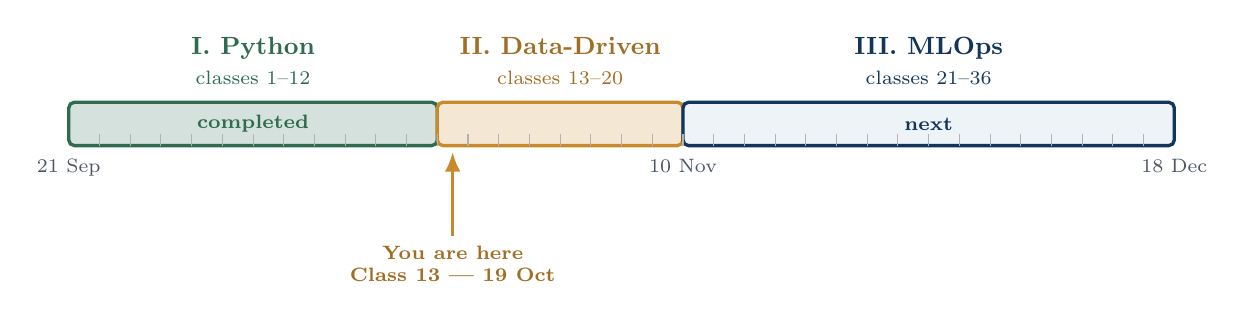
\begin{tikzpicture}[x=0.39cm, y=1cm]
% block bars (one unit per class)
\fill[coursegreen!20, draw=coursegreen, very thick, rounded corners=2pt] (0,0) rectangle (12,0.55);
\fill[coursegold!20, draw=coursegold, very thick, rounded corners=2pt] (12,0) rectangle (20,0.55);
\fill[courseice, draw=courseblue, very thick, rounded corners=2pt] (20,0) rectangle (36,0.55);
% class ticks
\foreach \i in {1,...,35} { \draw[gray!60] (\i,0) -- (\i,0.15); }
% block labels
\node[above, align=center, font=\small\bfseries, text=coursegreen] at (6,0.65) {I. Python \\ \scriptsize\normalfont classes 1--12};
\node[above, align=center, font=\small\bfseries, text=coursegold!80!black] at (16,0.65) {II. Data-Driven \\ \scriptsize\normalfont classes 13--20};
\node[above, align=center, font=\small\bfseries, text=courseblue] at (28,0.65) {III. MLOps \\ \scriptsize\normalfont classes 21--36};
% status inside bars
\node[font=\scriptsize\bfseries, text=coursegreen] at (6,0.275) {completed};
\node[font=\scriptsize\bfseries, text=courseblue] at (28,0.275) {next};
% dates
\foreach \x/\d in {0/21 Sep, 20/10 Nov, 36/18 Dec} {
  \node[below, font=\scriptsize, text=coursegray] at (\x,-0.05) {\d};
}
% you are here
\draw[-{Latex[length=2.5mm,width=2mm]}, very thick, draw=coursegold] (12.5,-1.15) -- (12.5,-0.08);
\node[below, font=\scriptsize\bfseries, text=coursegold!80!black, align=center] at (12.5,-1.15) {You are here \\ Class 13 --- 19 Oct};
\end{tikzpicture}

\vspace{0.6em}
\begin{columns}[T]
\column{0.31\textwidth}
{\small\bfseries\color{coursegreen} Done: the tool}\\
{\scriptsize Syntax, data structures, functions, OOP, pandas, plotting, first EDA, scikit-learn API.}
\column{0.31\textwidth}
{\small\bfseries\color{coursegold!80!black} Now: the data}\\
{\scriptsize Data types, encoding, feature engineering, modeling, online ML, serving.}
\column{0.31\textwidth}
{\small\bfseries\color{courseblue} Next: the system}\\
{\scriptsize Software engineering, requirements, agile, MLOps, CI/CD, monitoring, project.}
\end{columns}
\coursefooter
\end{frame}

\begin{frame}{Agenda}
\begin{itemize}
\item Why identifying data type comes before any modeling decision.
\item Tabular data: samples, features, and the independent and identically distributed (i.i.d.)\ assumption.
\item Time series data: order, timestamps, and temporal dependency.
\item Spectral and signal data: waveforms and frequency-domain thinking.
\item Image data: pixels, grids, and spatial structure.
\item How the fraud and pasteurization cases embody different data types.
\end{itemize}
\coursefooter
\end{frame}

\begin{frame}{Learning goals}
\learninggoals{
\begin{itemize}
\item Recognize that ``a dataset'' is not one thing: tabular, time series, spectral, and image data carry different assumptions.
\item Identify which assumptions (independence, ordering, locality) each data type licenses or forbids.
\item Connect each data type to a concrete artifact already in this repository.
\item Explain why data type must be settled before encoding, feature engineering, or model choice.
\end{itemize}
}
\coursefooter
\end{frame}
\begin{frame}{Why data type matters before modeling}
\begin{itemize}
\item Every learning algorithm carries an inductive bias, i.e.\ structural assumptions about the data: exchangeability of samples, serial dependence over time, or locality over a spatial domain.
\item Applying a method whose assumptions are violated by the data (e.g.\ an i.i.d.\ method on serially dependent observations) discards the very structure that carries the information.
\item Data type is a property of the data-generating process, not of the storage format: the same physical quantity (temperature) may constitute i.i.d.\ samples in one study and a time series in another.
\item Fixing the data type therefore constrains the admissible representations, feature constructions, and model families.
\end{itemize}
\coursefooter
\end{frame}

\begin{frame}{The i.i.d.\ assumption}
\begin{columns}[T]
\column{0.5\textwidth}
{\small\textbf{\color{courseblue} Independent:} $p(\mathbf{x}_i, \mathbf{x}_j) = p(\mathbf{x}_i)\,p(\mathbf{x}_j)$ for $i \neq j$; observing one sample conveys no information about another.}
\column{0.5\textwidth}
{\small\textbf{\color{courseblue} Identically distributed:} every sample is drawn from the same $p(\mathbf{x}, y)$; the generating process does not change across samples.}
\end{columns}
\vspace{0.4em}
\centering
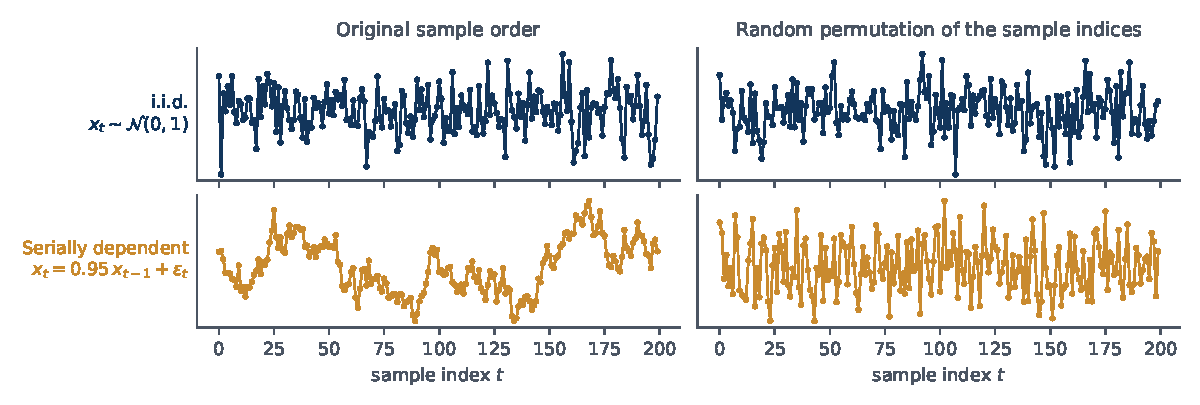
\includegraphics[width=\textwidth,height=0.5\textheight,keepaspectratio]{images/class13_iid_vs_dependent.pdf}

{\scriptsize Permutation test: under the i.i.d.\ assumption, a random permutation of the sample indices leaves the joint distribution unchanged (top); under serial dependence, the same permutation destroys the temporal structure (bottom).}
\coursefooter
\end{frame}

\begin{frame}{Tabular data versus time series under permutation}
\begin{columns}[T]
\column{0.5\textwidth}
{\small\textbf{\color{courseblue} Tabular:} the dataset is a multiset $\{(\mathbf{x}_i, y_i)\}_{i=1}^{n}$; estimators that depend only on the empirical distribution are invariant to permutations of the sample indices.}
\column{0.5\textwidth}
{\small\textbf{\color{coursegold!80!black} Time series:} the dataset is a sequence $(x_1, \dots, x_T)$; the order is part of the data, and quantities such as $\dot{T}(t)$ depend on it.}
\end{columns}
\vspace{0.3em}
\centering
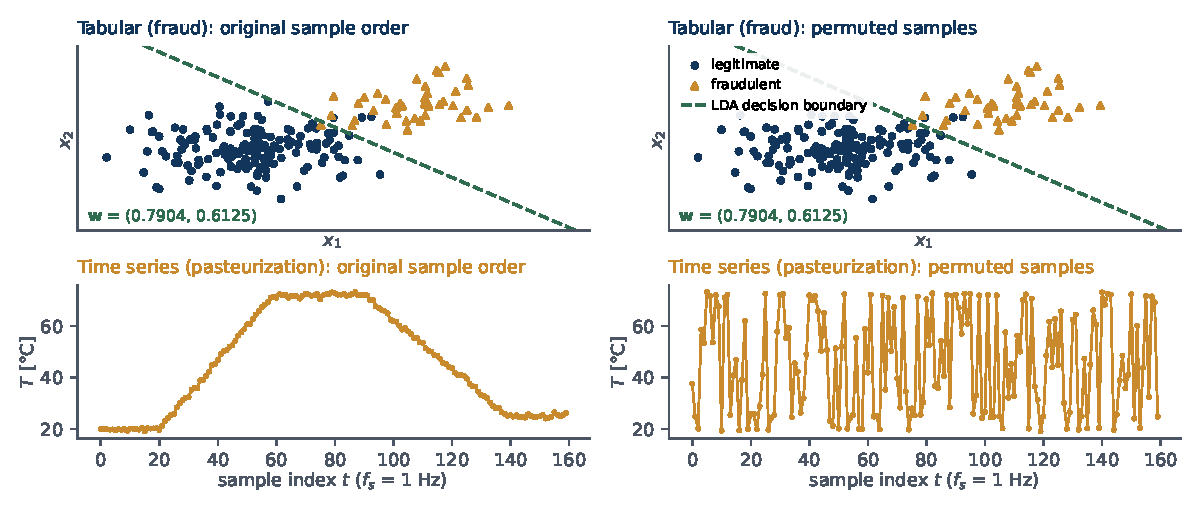
\includegraphics[width=\textwidth,height=0.5\textheight,keepaspectratio]{images/class13_tabular_vs_timeseries_shuffle.pdf}

{\scriptsize Top: the estimated linear discriminant $\mathbf{w}$ is identical before and after the permutation. Bottom: permuting the sensor record eliminates the heating, holding, and cooling phases.}
\coursefooter
\end{frame}

\begin{frame}{Notation}
\begin{itemize}
\item A supervised dataset is a collection of $n$ samples (instances, observations), possibly with repetitions:
\[
\mathcal{D} = \{(\mathbf{x}_i, y_i)\}_{i=1}^{n}, \qquad \mathbf{x}_i = (x_{i,1}, \dots, x_{i,d})^{\top} \in \mathcal{X} = \mathcal{X}_1 \times \dots \times \mathcal{X}_d, \quad y_i \in \mathcal{Y}.
\]
\item $x_{i,j} \in \mathcal{X}_j$ is the value of feature (attribute, variable) $j \in \{1,\dots,d\}$ for sample $i$, where $\mathcal{X}_j$ is the domain of feature $j$ (e.g.\ $\mathbb{R}$ or a finite set of categories); $y_i$ is the corresponding target.
\item Once all features are numerically encoded (Class 14), $\mathcal{X} \subseteq \mathbb{R}^{d}$ and the samples form the design matrix $X \in \mathbb{R}^{n \times d}$, whose $i$-th row is $\mathbf{x}_i^{\top}$ and whose $j$-th column collects feature $j$.
\item Features are classified by measurement scale (Stevens, 1946):
\begin{itemize}
\item \textbf{nominal} (categories without order), \textbf{ordinal} (ordered categories),
\item \textbf{interval} and \textbf{ratio} (numerical; continuous or discrete).
\end{itemize}
\end{itemize}
\coursefooter
\end{frame}

\begin{frame}{Single-target and multi-target problems}
\vspace{0.2em}{\small With $q > 1$ targets per sample, $\mathbf{y}_i = (y_{i1}, \dots, y_{iq}) \in \mathcal{Y}_1 \times \dots \times \mathcal{Y}_q$, and the targets form an $n \times q$ matrix $Y$.}
\vspace{0.4em}

{\footnotesize
\begin{tabularx}{\textwidth}{>{\bfseries}l >{\raggedright\arraybackslash}p{4.4cm} >{\raggedright\arraybackslash}X}
Problem & Target space & Example \\
\toprule
Binary classification & $y_i \in \{0, 1\}$ & Fraud detection (\texttt{is\_fraud}) \\
Multi-class classification & $y_i \in \{1, \dots, K\}$ & Process phase $s_t$, $K = 6$ \\
Multi-label classification & $\mathbf{y}_i \in \{0, 1\}^{q}$ & Concurrent alarms in a batch \\
Multi-target regression & $\mathbf{y}_i \in \mathbb{R}^{q}$ & Forecast of $T_{t+1}, \dots, T_{t+h}$ \\
\bottomrule
\end{tabularx}
}
\vspace{0.4em}
\begin{itemize}\footnotesize
\item \emph{Multi-output} and \emph{multi-target} are synonyms; multi-label classification is the special case $\mathcal{Y}_k = \{0, 1\}$.
\item Central issue: dependence among targets. Per-target models (binary relevance) ignore it; joint models (classifier chains, multivariate regression) exploit it.
\item Evaluation requires dedicated metrics, e.g.\ Hamming loss and subset accuracy.
\end{itemize}
\coursefooter
\end{frame}

\begin{frame}{Tabular data}
\begin{itemize}
\item Tabular data is represented by a design matrix $X \in \mathbb{R}^{n \times d}$ with a fixed, semantically meaningful feature set shared by all samples.
\item The standard assumption is that samples are independent and identically distributed:
\[
(\mathbf{x}_i, y_i) \overset{\text{i.i.d.}}{\sim} p(\mathbf{x}, y), \qquad i = 1,\dots,n.
\]
\item Consequence: the empirical risk is invariant to any permutation $\pi$ of the sample indices, so the order of samples carries no information.
\item Features may be heterogeneous in scale (nominal, ordinal, numerical), which motivates the encoding techniques of Class 14.
\item Most classical learning methods (linear models, decision-tree ensembles, $k$-NN, SVMs) are formulated under this assumption.
\end{itemize}
\coursefooter
\end{frame}

\begin{frame}{Tabular example: the fraud dataset}
\centering
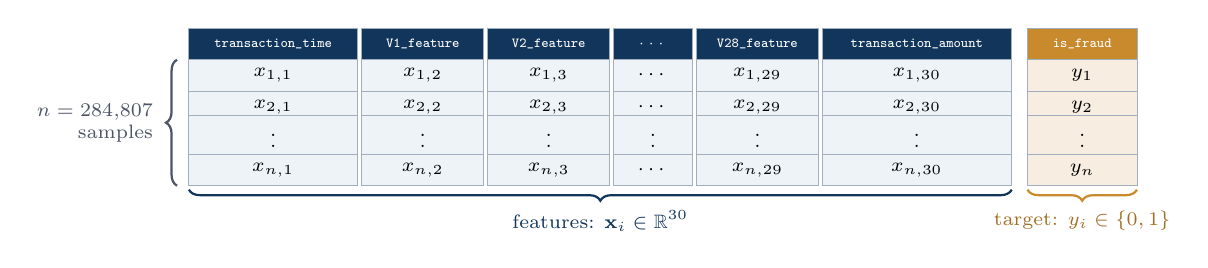
\begin{tikzpicture}[
  cell/.style={draw=courseblue!40, minimum height=0.4cm, font=\scriptsize, inner sep=1pt},
  head/.style={cell, fill=courseblue, text=white, font=\tiny\ttfamily},
  thead/.style={cell, fill=coursegold, text=white, font=\tiny\ttfamily}
]
\node[head, minimum width=2.15cm] at (0.0, 0) {transaction\_time};
\node[head, minimum width=1.55cm] at (1.9, 0) {V1\_feature};
\node[head, minimum width=1.55cm] at (3.5, 0) {V2\_feature};
\node[head, minimum width=1.0cm] at (4.825, 0) {$\cdots$};
\node[head, minimum width=1.55cm] at (6.15, 0) {V28\_feature};
\node[head, minimum width=2.4cm] at (8.175, 0) {transaction\_amount};
\node[thead, minimum width=1.4cm] at (10.275, 0) {is\_fraud};
\node[cell, fill=courseice, minimum width=2.15cm] at (0.0, -0.40) {$x_{1,1}$};
\node[cell, fill=courseice, minimum width=1.55cm] at (1.9, -0.40) {$x_{1,2}$};
\node[cell, fill=courseice, minimum width=1.55cm] at (3.5, -0.40) {$x_{1,3}$};
\node[cell, fill=courseice, minimum width=1.0cm] at (4.825, -0.40) {$\cdots$};
\node[cell, fill=courseice, minimum width=1.55cm] at (6.15, -0.40) {$x_{1,29}$};
\node[cell, fill=courseice, minimum width=2.4cm] at (8.175, -0.40) {$x_{1,30}$};
\node[cell, fill=coursegold!15, minimum width=1.4cm] at (10.275, -0.40) {$y_{1}$};
\node[cell, fill=courseice, minimum width=2.15cm] at (0.0, -0.80) {$x_{2,1}$};
\node[cell, fill=courseice, minimum width=1.55cm] at (1.9, -0.80) {$x_{2,2}$};
\node[cell, fill=courseice, minimum width=1.55cm] at (3.5, -0.80) {$x_{2,3}$};
\node[cell, fill=courseice, minimum width=1.0cm] at (4.825, -0.80) {$\cdots$};
\node[cell, fill=courseice, minimum width=1.55cm] at (6.15, -0.80) {$x_{2,29}$};
\node[cell, fill=courseice, minimum width=2.4cm] at (8.175, -0.80) {$x_{2,30}$};
\node[cell, fill=coursegold!15, minimum width=1.4cm] at (10.275, -0.80) {$y_{2}$};
\node[cell, fill=courseice, minimum width=2.15cm] at (0.0, -1.20) {$\vdots$};
\node[cell, fill=courseice, minimum width=1.55cm] at (1.9, -1.20) {$\vdots$};
\node[cell, fill=courseice, minimum width=1.55cm] at (3.5, -1.20) {$\vdots$};
\node[cell, fill=courseice, minimum width=1.0cm] at (4.825, -1.20) {$\vdots$};
\node[cell, fill=courseice, minimum width=1.55cm] at (6.15, -1.20) {$\vdots$};
\node[cell, fill=courseice, minimum width=2.4cm] at (8.175, -1.20) {$\vdots$};
\node[cell, fill=coursegold!15, minimum width=1.4cm] at (10.275, -1.20) {$\vdots$};
\node[cell, fill=courseice, minimum width=2.15cm] at (0.0, -1.60) {$x_{n,1}$};
\node[cell, fill=courseice, minimum width=1.55cm] at (1.9, -1.60) {$x_{n,2}$};
\node[cell, fill=courseice, minimum width=1.55cm] at (3.5, -1.60) {$x_{n,3}$};
\node[cell, fill=courseice, minimum width=1.0cm] at (4.825, -1.60) {$\cdots$};
\node[cell, fill=courseice, minimum width=1.55cm] at (6.15, -1.60) {$x_{n,29}$};
\node[cell, fill=courseice, minimum width=2.4cm] at (8.175, -1.60) {$x_{n,30}$};
\node[cell, fill=coursegold!15, minimum width=1.4cm] at (10.275, -1.60) {$y_{n}$};
\draw[decorate, decoration={brace, amplitude=4pt, mirror}, thick, courseblue] (-1.07,-1.85) -- (9.38,-1.85) node[midway, below=4pt, font=\scriptsize, text=courseblue] {features: $\mathbf{x}_i \in \mathbb{R}^{30}$};
\draw[decorate, decoration={brace, amplitude=4pt, mirror}, thick, coursegold] (9.58,-1.85) -- (10.97,-1.85) node[midway, below=4pt, font=\scriptsize, text=coursegold!80!black] {target: $y_i \in \{0,1\}$};
\draw[decorate, decoration={brace, amplitude=4pt}, thick, coursegray] (-1.22,-1.80) -- (-1.22,-0.2) node[midway, left=5pt, font=\scriptsize, text=coursegray, align=right] {$n = 284{,}807$\\samples};
\end{tikzpicture}

\vspace{0.4em}
{\scriptsize
\begin{tabularx}{\textwidth}{>{\ttfamily}l l >{\raggedright\arraybackslash}X l}
\normalfont\bfseries Feature & \bfseries Scale & \bfseries Description & \bfseries Summary \\
\toprule
transaction\_time & interval & Seconds elapsed since the first transaction & 0 -- 172{,}792\,s ($\approx$ 48\,h) \\
V1\_feature, \dots, V28\_feature & interval & Principal components of anonymized attributes & mean $\approx 0$; s.d.\ 1.96 (V1) to 0.33 (V28) \\
transaction\_amount & ratio & Monetary value of the transaction & median 22.00; max 25{,}691.16 \\
is\_fraud & nominal & Target: 1 if fraudulent, 0 otherwise & prevalence 0.173\% \\
\bottomrule
\end{tabularx}
}

\vspace{0.2em}
{\scriptsize Source: \texttt{Credit\_Card\_Fraud\_Detection\_Solution.ipynb}, output of \texttt{df.describe()}.}
\coursefooter
\end{frame}

\begin{frame}{A taxonomy of data types}
\begingroup\footnotesize
\begin{tabularx}{\textwidth}{>{\bfseries}l >{\raggedright\arraybackslash}X >{\raggedright\arraybackslash}X >{\raggedright\arraybackslash}X >{\raggedright\arraybackslash}X}
Data type & Index domain & Dependence structure & Expected invariance & Typical model families \\
\toprule
Tabular & None (sample set) & Independent samples & Permutation of samples & Linear models, tree ensembles, $k$-NN \\
\addlinespace[0.5em]
Time series & Time $t \in \{1,\dots,T\}$ & Serial dependence, $\rho(k) \neq 0$ & Shift in time (if stationary) & ARIMA, state-space models, RNNs \\
\addlinespace[0.5em]
Signal / spectrum & Time or frequency & Periodic components & Shift in time; phase & DFT/STFT features, 1D CNNs \\
\addlinespace[0.5em]
Image & Spatial grid $(u, v)$ & Local spatial correlation & Translation & CNNs, vision transformers \\
\bottomrule
\end{tabularx}
\endgroup
\vspace{0.6em}
\begin{itemize}
\item The invariance column states which transformations of the input should leave the prediction unchanged; it is what a well-chosen model family encodes by construction.
\end{itemize}
\coursefooter
\end{frame}

\begin{frame}{Time series data}
\begin{itemize}
\item A time series is a realization $\{x_t\}_{t=1}^{T}$ of a stochastic process indexed by time; the index is part of the data, not a storage artifact.
\item Observations exhibit serial dependence, quantified by the autocorrelation function
\[
\rho(k) = \frac{\operatorname{Cov}(x_t, x_{t-k})}{\operatorname{Var}(x_t)}, \qquad \rho(k) \neq 0 \text{ for small lags } k.
\]
\item A process is (weakly) stationary if its mean and autocovariance do not depend on $t$; trend, seasonality, and regime changes violate this.
\item Classical decomposition: $x_t = m_t + s_t + \varepsilon_t$ (trend, seasonal component, residual).
\item The i.i.d.\ assumption does not hold, so random resampling for model validation is not admissible.
\end{itemize}
\coursefooter
\end{frame}

\begin{frame}{Variance, covariance, and decomposition}
\centering
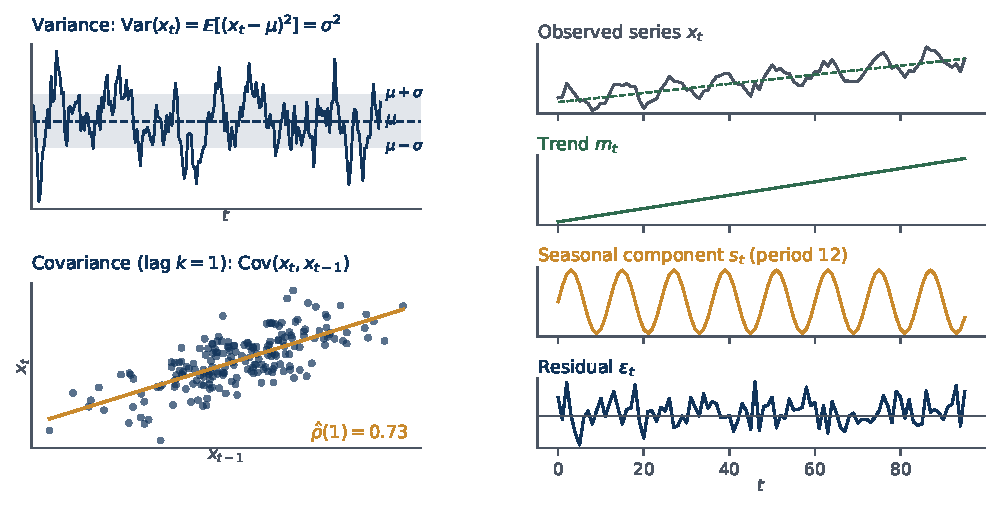
\includegraphics[width=\textwidth,height=0.72\textheight,keepaspectratio]{images/class13_ts_concepts.pdf}

\vspace{0.2em}
{\scriptsize Left: a stationary process, with $\rho(1) = \mathrm{Cov}(x_t, x_{t-1})/\sigma^2$. Right: additive decomposition $x_t = m_t + s_t + \varepsilon_t$.}
\coursefooter
\end{frame}

\begin{frame}{Time series example: a pasteurization batch}
\begin{columns}[T]
\column{0.57\textwidth}
\centering
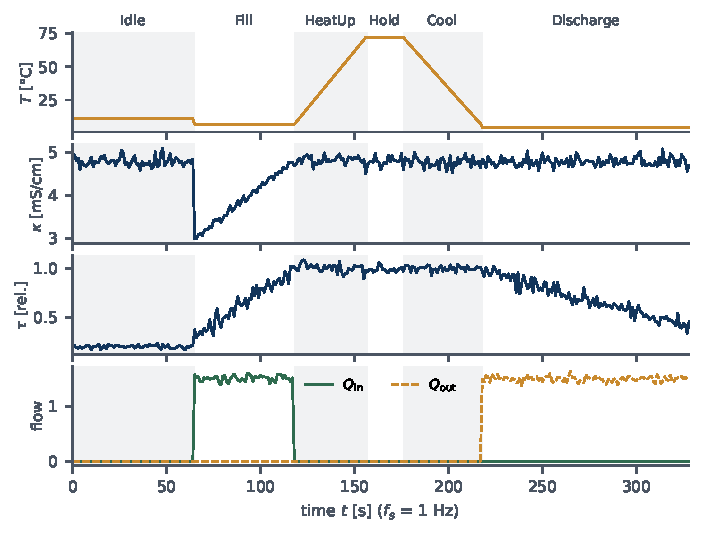
\includegraphics[width=\linewidth,height=0.68\textheight,keepaspectratio]{images/class13_pasteurization_batch.pdf}

{\tiny One batch from \texttt{synth\_sensors.py}; $\mathbf{x}_t \in \mathbb{R}^{8}$, four of the eight channels shown.}
\column{0.41\textwidth}
\begin{block}{Task}
\footnotesize
Given the window $W_t = (\mathbf{x}_{t-w+1}, \dots, \mathbf{x}_t)$, predict the process phase
\vspace{-0.3em}\[
s_t \in \mathcal{S} = \{\text{Idle}, \dots, \text{Discharge}\}.
\]
\begin{enumerate}\setlength{\itemsep}{1pt}
\item Classify the task by its target space.
\item Identify the channels that discriminate Fill from Discharge.
\item Explain why $\dot{T}(t) \approx (T_t - T_{t-1})/\Delta t$ is informative for HeatUp and Cool.
\item Propose a train/test split that is valid for this dataset.
\end{enumerate}
\end{block}
\end{columns}
\coursefooter
\end{frame}

\begin{frame}{From raw signal to derived feature}
\centering
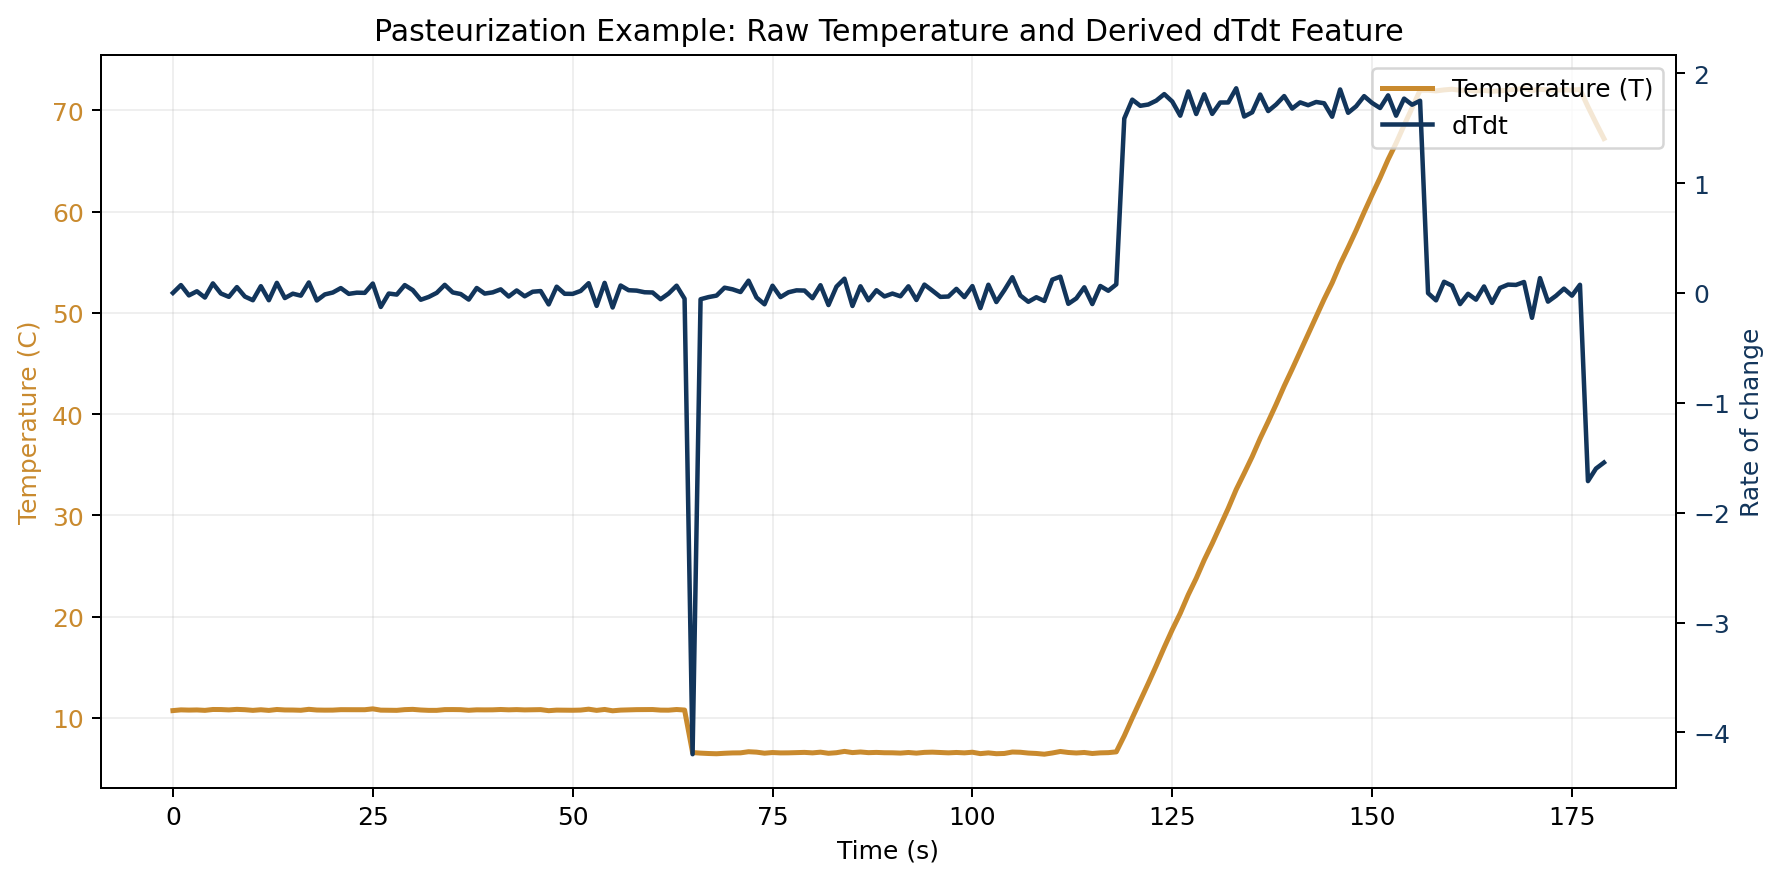
\includegraphics[height=0.72\textheight]{images/class04_pasteurization_dt_plot.png}

{\scriptsize Temperature $T_t$ and its finite-difference derivative $\dot{T}(t)$ from \texttt{pasteurization/synth\_sensors.py}: the derived feature makes the heating and cooling regimes explicit.}
\coursefooter
\end{frame}

\begin{frame}{Spectral and signal data}
\begin{itemize}
\item A discrete signal $x[n] = x(n/f_s)$ is obtained by sampling a continuous phenomenon at frequency $f_s$ (audio, vibration, high-rate sensors).
\item Nyquist--Shannon: a component of frequency $f$ is recoverable only if $f_s > 2 f_{\max}$; otherwise it is aliased onto lower frequencies.
\item The discrete Fourier transform (DFT) re-expresses a length-$N$ signal as a combination of $N$ frequency components.
\item Non-stationary signals are analysed with the short-time Fourier transform (windowed DFT); in speech, MFCCs summarize each window on a perceptual frequency scale.
\item The repository contains no audio dataset; the pasteurization temperature trace serves as the reference example of a sampled physical signal.
\end{itemize}
\coursefooter
\end{frame}

\begin{frame}{Spectroscopic data: NIRS and X-ray}
\centering
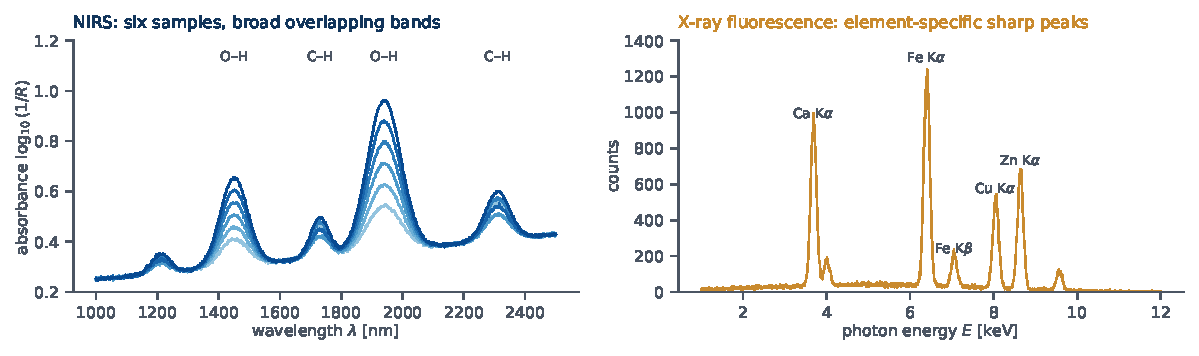
\includegraphics[width=\textwidth,height=0.4\textheight,keepaspectratio]{images/class13_nirs_xrf_spectra.pdf}

\vspace{0.2em}
\begin{itemize}\footnotesize
\item Each sample is a spectrum $\mathbf{x}_i = (x_i(\lambda_1), \dots, x_i(\lambda_d))$ indexed by wavelength or energy, not by time; adjacent variables are strongly correlated and typically $d \gg n$.
\item \textbf{Near-infrared spectroscopy (NIRS)}, 780--2500\,nm: broad, overlapping overtone and combination bands of O--H, C--H, and N--H bonds; used to estimate composition (moisture, fat, protein). Standard pipeline: scatter correction (SNV, MSC), Savitzky--Golay derivatives, partial least squares (PLS) regression.
\item \textbf{X-ray spectroscopy}: fluorescence (XRF) yields sharp peaks at element-specific energies (elemental composition); diffraction (XRD) yields peaks over the angle $2\theta$ (crystalline phases). X-ray radiographs, by contrast, are images.
\end{itemize}
\vspace{-0.3em}
{\tiny Illustrative synthetic spectra; band and line positions follow standard reference values.}
\coursefooter
\end{frame}

\begin{frame}{Time series versus spectral data}
\centering
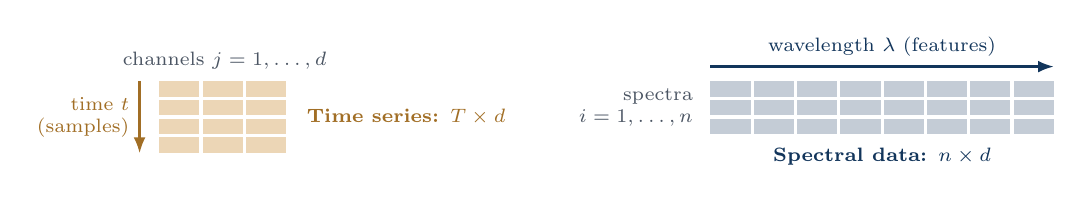
\begin{tikzpicture}
\fill[coursegold!35] (0.00,0.00) rectangle ++(0.51,-0.20);
\fill[coursegold!35] (0.55,0.00) rectangle ++(0.51,-0.20);
\fill[coursegold!35] (1.10,0.00) rectangle ++(0.51,-0.20);
\fill[coursegold!35] (0.00,-0.24) rectangle ++(0.51,-0.20);
\fill[coursegold!35] (0.55,-0.24) rectangle ++(0.51,-0.20);
\fill[coursegold!35] (1.10,-0.24) rectangle ++(0.51,-0.20);
\fill[coursegold!35] (0.00,-0.48) rectangle ++(0.51,-0.20);
\fill[coursegold!35] (0.55,-0.48) rectangle ++(0.51,-0.20);
\fill[coursegold!35] (1.10,-0.48) rectangle ++(0.51,-0.20);
\fill[coursegold!35] (0.00,-0.72) rectangle ++(0.51,-0.20);
\fill[coursegold!35] (0.55,-0.72) rectangle ++(0.51,-0.20);
\fill[coursegold!35] (1.10,-0.72) rectangle ++(0.51,-0.20);
\draw[-{Latex[length=2mm]}, thick, coursegold!80!black] (-0.25,0) -- (-0.25,-0.92) node[midway, left, font=\scriptsize, align=right] {time $t$\\(samples)};
\node[font=\scriptsize, text=coursegray, above] at (0.83,0.02) {channels $j = 1,\dots,d$};
\node[font=\scriptsize\bfseries, text=coursegold!80!black, right] at (1.75,-0.46) {Time series: $T \times d$};
\fill[courseblue!25] (7.00,0.00) rectangle ++(0.51,-0.20);
\fill[courseblue!25] (7.55,0.00) rectangle ++(0.51,-0.20);
\fill[courseblue!25] (8.10,0.00) rectangle ++(0.51,-0.20);
\fill[courseblue!25] (8.65,0.00) rectangle ++(0.51,-0.20);
\fill[courseblue!25] (9.20,0.00) rectangle ++(0.51,-0.20);
\fill[courseblue!25] (9.75,0.00) rectangle ++(0.51,-0.20);
\fill[courseblue!25] (10.30,0.00) rectangle ++(0.51,-0.20);
\fill[courseblue!25] (10.85,0.00) rectangle ++(0.51,-0.20);
\fill[courseblue!25] (7.00,-0.24) rectangle ++(0.51,-0.20);
\fill[courseblue!25] (7.55,-0.24) rectangle ++(0.51,-0.20);
\fill[courseblue!25] (8.10,-0.24) rectangle ++(0.51,-0.20);
\fill[courseblue!25] (8.65,-0.24) rectangle ++(0.51,-0.20);
\fill[courseblue!25] (9.20,-0.24) rectangle ++(0.51,-0.20);
\fill[courseblue!25] (9.75,-0.24) rectangle ++(0.51,-0.20);
\fill[courseblue!25] (10.30,-0.24) rectangle ++(0.51,-0.20);
\fill[courseblue!25] (10.85,-0.24) rectangle ++(0.51,-0.20);
\fill[courseblue!25] (7.00,-0.48) rectangle ++(0.51,-0.20);
\fill[courseblue!25] (7.55,-0.48) rectangle ++(0.51,-0.20);
\fill[courseblue!25] (8.10,-0.48) rectangle ++(0.51,-0.20);
\fill[courseblue!25] (8.65,-0.48) rectangle ++(0.51,-0.20);
\fill[courseblue!25] (9.20,-0.48) rectangle ++(0.51,-0.20);
\fill[courseblue!25] (9.75,-0.48) rectangle ++(0.51,-0.20);
\fill[courseblue!25] (10.30,-0.48) rectangle ++(0.51,-0.20);
\fill[courseblue!25] (10.85,-0.48) rectangle ++(0.51,-0.20);
\draw[-{Latex[length=2mm]}, thick, courseblue] (7.00,0.18) -- (11.36,0.18) node[midway, above, font=\scriptsize] {wavelength $\lambda$ (features)};
\node[font=\scriptsize, text=coursegray, left, align=right] at (6.90,-0.34) {spectra\\$i = 1,\dots,n$};
\node[font=\scriptsize\bfseries, text=courseblue, below] at (9.18,-0.73) {Spectral data: $n \times d$};
\end{tikzpicture}

\vspace{0.1em}
\begingroup\scriptsize
\begin{tabularx}{\textwidth}{>{\bfseries}l >{\raggedright\arraybackslash}X >{\raggedright\arraybackslash}X}
& \bfseries Time series & \bfseries Spectral data (e.g.\ NIRS) \\
\toprule
Index & Time $t$; indexes the samples & Wavelength $\lambda$ or energy $E$; indexes the features (spectra are usually i.i.d.) \\
Direction & Causal: the past determines the future & Non-causal: no preferred direction, two-sided filters are admissible \\
Typical question & Forecasting $x_{t+h}$, detecting regime changes & Predicting a property $y_i$ from the whole spectrum \\
Valid split & Temporal (train before test) & By physical sample (replicates kept together) \\
\bottomrule
\end{tabularx}
\endgroup

\vspace{0.4em}
\begin{itemize}\footnotesize
\item \textbf{Common ground:} both are functions sampled on an ordered grid, with strong correlation between neighbouring points.
\item \textbf{Relation:} the Fourier transform maps a time series to its frequency spectrum; FT-NIR instruments obtain spectra by Fourier-transforming a measured interferogram.
\end{itemize}
\coursefooter
\end{frame}

\begin{frame}{Image data}
\begin{itemize}
\item An image is a tensor $I \in \mathbb{R}^{H \times W \times C}$ ($C = 1$ for grayscale, $C = 3$ for red--green--blue (RGB) channels), i.e.\ a function on a discrete spatial grid $(u, v)$.
\item Spatial locality: correlation between pixels decays with their distance, so relevant patterns are local.
\item Semantic content is (approximately) invariant to translation; convolution is translation-equivariant, $f(\tau_{\delta} I) = \tau_{\delta} f(I)$, which motivates convolutional neural networks (CNNs).
\item The index domain is two-dimensional and has no natural total order: flattening to a vector of length $H \cdot W \cdot C$ discards the neighborhood structure.
\item The repository contains no image dataset; the type is included to complete the taxonomy before representation is discussed in Class 14.
\end{itemize}
\coursefooter
\end{frame}

\begin{frame}{Consequences of ignoring the data type}
\begin{tabularx}{\textwidth}{>{\bfseries}l X}
Data type & Assumption violated by a naive tabular treatment \\
\toprule
Time series & Exchangeability: random splits place future samples in the training set (temporal leakage). \\
Signal / spectrum & Representation: raw amplitudes in the time domain obscure the periodic components, which are sparse in the frequency domain. \\
Image & Locality: flattening to $\mathbb{R}^{H \cdot W \cdot C}$ discards spatial neighborhoods and translation structure. \\
\bottomrule
\end{tabularx}
\coursefooter
\end{frame}

\begin{frame}{Data leakage and valid evaluation}
\vspace{-0.4em}\begingroup\footnotesize \textbf{Definition:} leakage occurs when information that would be unavailable at prediction time influences model training or model selection, yielding optimistically biased performance estimates.\par\endgroup
\vspace{0.2em}

\begingroup\scriptsize
\begin{tabularx}{\textwidth}{>{\bfseries\raggedright\arraybackslash}p{2.3cm} >{\raggedright\arraybackslash}X >{\raggedright\arraybackslash}X >{\raggedright\arraybackslash}X}
Type & Mechanism & Example & Remedy \\
\toprule
Target leakage & A feature encodes the target or is recorded after it & A chargeback flag used to predict \texttt{is\_fraud} & Retain only features available at prediction time \\
\addlinespace[0.35em]
Preprocessing contamination & Transformations fitted before splitting & Scaling, imputation, PCA, or oversampling fitted on all data & Fit transformations on the training fold only (pipeline) \\
\addlinespace[0.35em]
Temporal leakage & Future observations inform the past & Random $k$-fold on the sensor log; centred rolling means & $\max t_{\text{train}} < \min t_{\text{test}}$; rolling origin; causal features \\
\addlinespace[0.35em]
Group leakage & Samples of one entity on both sides of the split & Windows of one batch; replicate spectra of one sample & Group-wise split \\
\addlinespace[0.35em]
Duplicate leakage & (Near-)identical samples in train and test & Repeated transactions or re-measured spectra & Deduplicate before splitting \\
\addlinespace[0.35em]
Model-selection leakage & The test set guides tuning or feature selection & Hyperparameters chosen by test-set error & Validation set or nested cross-validation \\
\bottomrule
\end{tabularx}
\endgroup
\coursefooter
\end{frame}

\begin{frame}{From data type to system design}
\centering
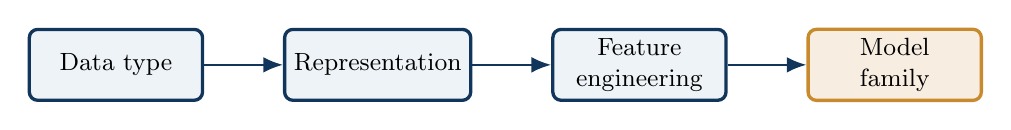
\begin{tikzpicture}[node distance=1cm and 1cm]
\node[flowbox] (type) {Data type};
\node[flowbox, right=of type] (rep) {Representation};
\node[flowbox, right=of rep] (feat) {Feature\\engineering};
\node[accentbox, right=of feat] (model) {Model\\family};
\draw[arrow] (type) -- (rep);
\draw[arrow] (rep) -- (feat);
\draw[arrow] (feat) -- (model);
\end{tikzpicture}
\vspace{0.5em}
\begin{itemize}
\item Each stage is the subject of a subsequent class: representation and encoding (Class 14), feature engineering (Class 15), and modeling (Class 16).
\item An error at the first stage propagates to every subsequent stage of the pipeline.
\end{itemize}
\coursefooter
\end{frame}

\begin{frame}{Repository connections}
\repoactivity{
\begin{itemize}
\item \texttt{Credit\_Card\_Fraud\_Detection\_Solution.ipynb} and \texttt{streamlit/modeling.py}: tabular data, one sample per transaction.
\item \texttt{pasteurization/synth\_sensors.py}: multivariate time series, eight sensor channels sampled at 1\,Hz over a batch lifecycle.
\item \texttt{pasteurization/serving.py}: the same process delivered as a data stream, used in the practical session of Class 19.
\end{itemize}
}
\coursefooter
\end{frame}

\begin{frame}{Common methodological errors}
\begin{itemize}
\item Treating a time-ordered sensor log as an i.i.d.\ sample and randomly permuting it before the train/test split.
\item Interpreting feature-importance measures computed on raw pixels as if pixels were semantically meaningful features.
\item Sampling below the Nyquist rate, so that the frequencies of interest are aliased and irrecoverable.
\item Equating sample size with information: under serial dependence the effective sample size is smaller than $n$.
\end{itemize}
\coursefooter
\end{frame}

\begin{frame}{Papers and materials}
\readinglist{
\fontsize{6.8}{8.2}\selectfont
\begin{columns}[T]
\column{0.5\textwidth}
\begin{itemize}\setlength{\itemsep}{1pt}
\item Stevens, S.\,S. (1946). On the theory of scales of measurement. \emph{Science}, 103(2684), 677--680.
\item Tsoumakas, G., Katakis, I. (2007). Multi-label classification: An overview. \emph{International Journal of Data Warehousing and Mining}, 3(3), 1--13.
\item Borchani, H., Varando, G., Bielza, C., Larra\~naga, P. (2015). A survey on multi-output regression. \emph{WIREs Data Mining and Knowledge Discovery}, 5(5), 216--233.
\item Hastie, T., Tibshirani, R., Friedman, J. (2009). \emph{The Elements of Statistical Learning}, 2nd ed. Springer.
\item Box, G.\,E.\,P., Jenkins, G.\,M., Reinsel, G.\,C., Ljung, G.\,M. (2015). \emph{Time Series Analysis: Forecasting and Control}, 5th ed. Wiley.
\item Oppenheim, A.\,V., Schafer, R.\,W. (2010). \emph{Discrete-Time Signal Processing}, 3rd ed. Pearson.
\end{itemize}
\column{0.5\textwidth}
\begin{itemize}\setlength{\itemsep}{1pt}
\item Workman, J., Weyer, L. (2012). \emph{Practical Guide and Spectral Atlas for Interpretive Near-Infrared Spectroscopy}, 2nd ed. CRC Press.
\item Wold, S., Sj\"ostr\"om, M., Eriksson, L. (2001). PLS-regression: a basic tool of chemometrics. \emph{Chemometrics and Intelligent Laboratory Systems}, 58(2), 109--130.
\item Goodfellow, I., Bengio, Y., Courville, A. (2016). \emph{Deep Learning}, ch.~9. MIT Press. \href{https://www.deeplearningbook.org}{deeplearningbook.org}
\item Kaufman, S., Rosset, S., Perlich, C., Stitelman, O. (2012). Leakage in data mining: Formulation, detection, and avoidance. \emph{ACM Transactions on Knowledge Discovery from Data}, 6(4), 1--21.
\item Kapoor, S., Narayanan, A. (2023). Leakage and the reproducibility crisis in machine-learning-based science. \emph{Patterns}, 4(9), 100804.
\item Huyen, C. (2022). \emph{Designing Machine Learning Systems}. O'Reilly.
\end{itemize}
\end{columns}
}
\coursefooter
\end{frame}

\begin{frame}{Take-away message}
\vfill
\centering
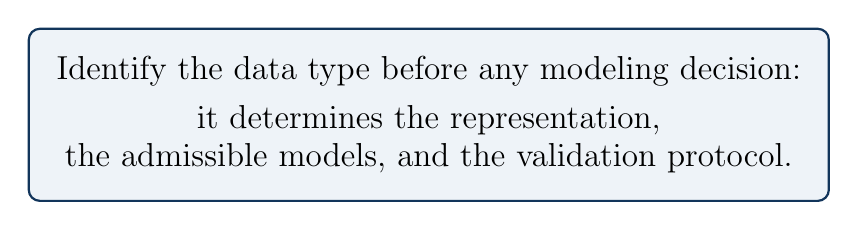
\begin{tikzpicture}
\node[fill=courseice, draw=courseblue, thick, rounded corners=4pt, inner sep=10pt, text width=0.78\textwidth, align=center, font=\large] {Identify the data type before any modeling decision:\\[0.3em] it determines the representation,\\ the admissible models, and the validation protocol.};
\end{tikzpicture}

\vfill
{\Large\bfseries\color{courseblue} Thank you for your attention.}

\vspace{0.4em}
{\small\color{coursegray} Next: Class 14 --- structured, semi-structured, and unstructured data; encoding and embedding.}
\vfill
\coursefooter
\end{frame}

\end{document}
